\subsection{Oscilações betatron pseudo-harmônicas}
As equações \eqref{eq:2.43} e \eqref{eq:2.44} descrevem completamente o caminho realizado pelo elétron. Para ter uma visão completa do movimento do elétron, basta apenas adicionar o fato de que o elétron viaja sempre na velocidade $c$ da luz. Fazendo uma aproximação, é adequado tomar que a coordenada longitudinal $s$ varia simplesmente como
	
\begin{align}
	s = s_0 + ct\label{eq:2.48}
\end{align}
	
A forma correta da equação \eqref{eq:2.48} será discutida na Seção \ref{sec:3.2}.
	
A função betatron descreve completamente as propriedades laterais de focalização do campo guia. Pela sua natureza, a função betatron deve ser sempre positiva definida, e sua curva tem uma forma semelhante a uma onda. Ela também é periódica ao longo do anel, logo
	
\begin{align}
	\beta(s+L) = \beta(s)
\end{align}
	
A função betatron possui um valor único em cada coordenada $s$. Se o campo guia é dividido em células idênticas (desconsiderando imperfeições de construção), $\beta$ terá a mesma simetria.
	
Conforme o elétron viaja ao redor do anel, ele executa uma oscilação lateral que não é nem harmônica e nem periódica. O movimento é um tipo de onda senoidal (\ref{fig:fig12}) distorcida com uma amplitude $a\sqrt{\beta}$ variante, a qual é modulada proporcionalmente à raiz da função betatron e com uma fase $(\varphi-\upsilon)$ que avança com $s$ a uma taxa de variação proporcional a $\frac{1}{\beta}$.
	
\begin{figure}[!htb]
	\centering
	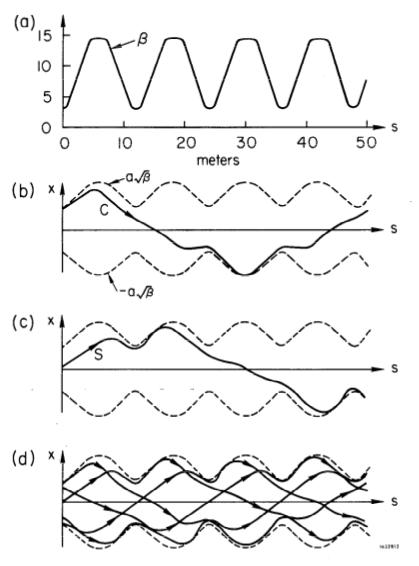
\includegraphics[width=0.7\linewidth]{./Figuras/fig12.jpeg}
	\caption{(a) Função betatron. (b) \textit{Cosine-like trajectory} para $s=0$. (c) \textit{Sine-like trajectory} para $s=0$. (d) Uma trajetória depois de várias revoluções sucessivas. Retirado de \cite{sands1970physics}.}
	\label{fig:fig12}
\end{figure}
	
Uma importante propriedade do movimento betatron é evidente na \ref{fig:fig12}(d) -- em cada coordenada, o desvio $x$ de um elétron em movimento fica sempre abaixo de um valor limitante $X(s)$, o qual é obtido colocando $cos(\varphi-\upsilon)=1$, ou seja,
	
\begin{align}
	X(s) = a\sqrt{\beta(s)}
\end{align}
	
A trajetória completa de um elétron armazenado cairá sempre dentro de um envelope definido por $\pm X(s)$. Segue que a abertura necessária para conter um elétron com uma amplitude de oscilação que varia ao redor do anel varia como $X(s)$. A relação entre a largura do envelope em duas coordenadas $s_1$ e $s_2$ é
	
\begin{align}
	\frac{X_2}{X_1} = \sqrt{\frac{\beta_2}{\beta_1}}
\end{align}
	
Para analisar a inclinação da trajetória betatron, ou seja, $x'=\frac{dx}{ds}$, considera-se a derivada da equação \eqref{eq:2.43}:
	
\begin{align}
	x' = - \frac{a}{\sqrt{\beta}}sen(\varphi-\upsilon)+\frac{\beta'}{2\beta}x\label{eq:2.52}
\end{align}
	
O primeiro termo vem da mudança de fase, e o segundo da variação de $\beta$.
	
\begin{proof}
	Seja $x(s) = a\sqrt{\beta(s)}\ cos\{\varphi(s)-\upsilon\}$. Logo, 
	\begin{align*}
      x' &= [a\sqrt{\beta}\ cos\{\varphi-\upsilon\}]'\\
         &= a[(\sqrt{\beta})'cos(\varphi-\upsilon)-\sqrt{\beta}\varphi'sen(\varphi-\upsilon)]\\
      	 &= a\left[\frac{\beta'}{2\sqrt{\beta}}cos(\varphi-\upsilon)-\sqrt{\beta}\frac{1}{\beta}sen(\varphi-\upsilon)\right]\\
      	 &= a\left[\frac{\beta'}{2\sqrt{\beta}}cos(\varphi-\upsilon)-\frac{1}{\sqrt{\beta}}sen(\varphi-\upsilon)\right]\\
      	 &= \frac{\beta'}{2\sqrt{\beta}}a\ cos(\varphi-\upsilon)-\frac{a}{\sqrt{\beta}}sen(\varphi-\upsilon)\\
      	 &= \frac{\beta'}{2\beta}a\sqrt{\beta}\ cos(\varphi-\upsilon)-\frac{a}{\sqrt{\beta}}sen(\varphi-\upsilon)\\
      	 &= -\frac{a}{\sqrt{\beta}}sen(\varphi-\upsilon)+\frac{\beta'}{2\beta}x
	\end{align*}
\end{proof}
	
Note que os zeros de $x'$ -- e, portanto, os valores de pico de $x$ -- não ocorrem em $cos(\varphi-\upsilon)=1$. Eles ocorrem em
	
\begin{align}
	tg(\varphi-\upsilon) = \frac{\beta'}{2}
\end{align}
o que significa que
\begin{align}
	cos(\varphi-\upsilon) = \left[1+\frac{\beta'^2}{4}\right]^{-\frac{1}{2}}
\end{align}
	
\begin{proof}
	Fazendo $x'=0$:
	\begin{align*}
        x'&=0\\
        -\frac{a}{\sqrt{\beta}}sen(\varphi-\upsilon)+\frac{\beta'}{2\beta}x &= 0\\
        \frac{\beta'}{2\beta}x &= \frac{a}{\sqrt{\beta}}sen(\varphi-\upsilon)\\
        \frac{\beta'}{2\beta}a\sqrt{\beta}\ cos\{\varphi-\upsilon\} &= \frac{a}{\sqrt{\beta}}sen(\varphi-\upsilon)\\
        \frac{\beta'}{2\beta}\sqrt{\beta}\sqrt{\beta} &= \frac{a}{a}\frac{sen(\varphi-\upsilon)}{cos(\varphi-\upsilon)}\\
        \frac{\beta'}{2} &= tg(\varphi-\upsilon)
	\end{align*}
	
	Pela identidade trigonométrica $1+tg^2(x) = sec^2(x)$,
	\begin{align*}
        1+tg^2(\varphi-\upsilon) &= sec^2(\varphi-\upsilon)\\
        1+\left(\frac{\beta'}{2}\right)^2 &= \left(\frac{1}{cos(\varphi-\upsilon)}\right)^2\\
        1+\frac{\beta'^2}{4} &= \frac{1}{cos^2(\varphi-\upsilon)}\\
        cos^2(\varphi-\upsilon) &= \left[1+\frac{\beta'^2}{4}\right]^{-1}\\
        cos(\varphi-\upsilon) &= \left[1+\frac{\beta'^2}{4}\right]^{-\frac{1}{2}}
	\end{align*}
	c.q.d.
\end{proof}
	
Se o pico de um ciclo particular de uma oscilação ocorrer em algum $s$, o valor de pico do desvio será
	
\begin{align}
	x_{pico} = a\sqrt{\beta}\left[1+\frac{\beta'^2}{4}\right]^{-\frac{1}{2}}
\end{align}
	
Em uma oscilação harmônica clássica, a amplitude é uma invariante do movimento. Seu quadrado é proporcional à energia da oscilação, e pode ser expresso como uma função quadrática da posição e velocidade instantâneas. O invariante correspondente do oscilador pseudo-harmônico é a constante $a$, e esta pode ser obtida em termos de $x$ e $x'$ pela equação
	
\begin{align}
	a^2 = \frac{x^2}{\beta} + \beta\left[x'-\frac{\beta'}{2\beta}x\right]^2\label{eq:2.56}
\end{align}
	
\begin{proof}
	Pela equação \eqref{eq:2.43},
	\begin{align*}
        x &= a\sqrt{\beta}\ cos\{\varphi-\upsilon\}\\
        \frac{x}{a\sqrt{\beta}} &= cos(\varphi-\upsilon)\\
        \left(\frac{x}{a\sqrt{\beta}}\right)^2 &= cos^2(\varphi-\upsilon)\\
        \frac{x^2}{a^2\beta} &= cos^2(\varphi-\upsilon)
	\end{align*}
	
	Já pela equação \eqref{eq:2.52},
	\begin{align*}
        x' &= - \frac{a}{\sqrt{\beta}}sen(\varphi-\upsilon)+\frac{\beta'}{2\beta}x\\
        x' - \frac{\beta'}{2\beta}x&= - \frac{a}{\sqrt{\beta}}sen(\varphi-\upsilon)\\
        \frac{\sqrt{\beta}}{a}\left[x' - \frac{\beta'}{2\beta}x\right]&= -sen(\varphi-\upsilon)\\
        \left(\frac{\sqrt{\beta}}{a}\left[x' - \frac{\beta'}{2\beta}x\right]\right)^2&= sen^2(\varphi-\upsilon)\\
        \frac{\beta}{a^2}\left[x' - \frac{\beta'}{2\beta}x\right]^2&= sen^2(\varphi-\upsilon)
	\end{align*}
	
	Pela relação trigonométrica $sen^2(x)+cos^2(x)=1$,
	\begin{align*}
        sen^2(\varphi-\upsilon)+cos^2(\varphi-\upsilon)&=1\\
        \frac{\beta}{a^2}\left[x' - \frac{\beta'}{2\beta}x\right]^2 + \frac{x^2}{a^2\beta} &= 1\\
        \frac{1}{a^2}\left(\beta\left[x' - \frac{\beta'}{2\beta}x\right]^2 + \frac{x^2}{\beta}\right) &= 1\\
        \beta\left[x' - \frac{\beta'}{2\beta}x\right]^2 + \frac{x^2}{\beta} &= a^2
	\end{align*}
	c.q.d.
\end{proof}
	
Se os valores de $x$ e $x'$ são conhecidos em alguma coordenada, supõe-se $s_1$, então a constante $a$ pode ser obtida e todos os valores subsequentes de $x$ e $x'$ podem ser expressos por
	
\begin{align}
	x = \frac{1}{\sqrt{\beta_1}}\left[x_1^2+\left(\beta_1x'_1-\frac{x_1\beta'_1}{2}\right)^2\right]^\frac{1}{2}\sqrt{\beta}\ cos(\varphi-\upsilon)\label{eq:2.57}
\end{align}
	
\begin{proof}
	Pela equação \eqref{eq:2.56},
	\begin{align*}
        a^2 &= \frac{x^2}{\beta} + \beta\left[x'-\frac{\beta'}{2\beta}x\right]^2\\
        	&= \frac{1}{\beta}\left(x^2 + \beta^2\left[x'-\frac{\beta'}{2\beta}x\right]^2\right)\\
        	&= \frac{1}{\beta}\left(x^2 + \left[\beta x'-\frac{\beta'}{2}x\right]^2\right)\\
        \therefore a &= \left[\frac{1}{\beta}\left(x^2 + \left[\beta x'-\frac{\beta'}{2}x\right]^2\right)\right]^\frac{1}{2}\\
        	&= \frac{1}{\sqrt{\beta}}\left(x^2 + \left[\beta x'-\frac{\beta'}{2}x\right]^2\right)^\frac{1}{2}
	\end{align*}
	
	Sejam $x(s_1)=x_1$, $x'(s_1)=x'_1$ e $\beta(s_1)=\beta_1$ os valores de $x$, $x'$ e $\beta$ conhecidos no ponto $s_1$, então $a$ pode ser determinado com estes valores:
	\begin{align*}
		a = \frac{1}{\sqrt{\beta_1}}\left(x_1^2 + \left[\beta_1 x_1'-\frac{\beta_1'}{2}x_1\right]^2\right)^\frac{1}{2}
	\end{align*}
	
	Substituindo o valor de $a$ na equação \eqref{eq:2.43},
	\begin{align*}
		x &= a\sqrt{\beta}\ cos\{\varphi-\upsilon\}\\
		  &= \frac{1}{\sqrt{\beta_1}}\left[x_1^2+\left(\beta_1x'_1-\frac{x_1\beta'_1}{2}\right)^2\right]^\frac{1}{2}\sqrt{\beta}\ cos(\varphi-\upsilon)
	\end{align*}
	c.q.d.
\end{proof}
	
A constante de fase $\upsilon$ também precisa ser determinada de $x$ e $x'$, e esta pode ser obtida pela equação
	
\begin{align}
	tg(\varphi_1 - \upsilon) = -\frac{\beta_1 x'_1}{x_1}+\frac{\beta'_1}{2}
\end{align}
onde $\varphi_1 = \varphi(s_1)$.
	
\begin{proof}
	Já foi deduzido anteriormente que
	\begin{align*}
        sen(\varphi-\upsilon) &= -\frac{\sqrt{\beta}}{a}\left[x' - \frac{\beta'}{2\beta}x\right]\\
        cos(\varphi-\upsilon) &= \frac{x}{a\sqrt{\beta}}
	\end{align*}
	
	Para obter $tg(\varphi-\upsilon)$, basta
	\begin{align*}
		tg(\varphi-\upsilon) &= \frac{sen(\varphi-\upsilon)}{cos(\varphi-\upsilon)}\\
							 &= \frac{-\frac{\sqrt{\beta}}{a}\left[x' - \frac{\beta'}{2\beta}x\right]}{\frac{x}{a\sqrt{\beta}}}\\
							 &= -\frac{\sqrt{\beta}}{a}\left[x' - \frac{\beta'}{2\beta}x\right] \frac{a\sqrt{\beta}}{x}\\
							 &= \frac{\beta}{x}\left[-x' + \frac{\beta'}{2\beta}x\right]\\
							 &= -\frac{\beta x'}{x} + \frac{\beta'}{2}\\
		\therefore tg(\varphi_1-\upsilon) &= -\frac{\beta_1  x_1'}{x_1} + \frac{\beta_1'}{2}
	\end{align*}
	
	Isolando $\upsilon$, pode-se obtê-lo diretamente pela relação
	\begin{align*}
		tg(\varphi_1-\upsilon) &= -\frac{\beta_1  x_1'}{x_1} + \frac{\beta_1'}{2}\\
		cotg(tg(\varphi_1-\upsilon)) &= cotg\left(-\frac{\beta_1  x_1'}{x_1} + \frac{\beta_1'}{2}\right)\\
		\varphi_1-\upsilon &= cotg\left(-\frac{\beta_1  x_1'}{x_1} + \frac{\beta_1'}{2}\right)\\
		\upsilon &= \varphi_1 - cotg\left(-\frac{\beta_1  x_1'}{x_1} + \frac{\beta_1'}{2}\right)
	\end{align*}
\end{proof}
	
Para obter o valor máximo $X(s)$ que pode ser alcançado em qualquer $s$ em qualquer revolução subsequente, basta substituir $cos(\varphi-\upsilon)=1$ na equação \eqref{eq:2.57}:
	
\begin{align}
	X(s) = \frac{1}{\sqrt{\beta_1}}\left[x_1^2+\left(\beta_1x'_1-\frac{x_1\beta'_1}{2}\right)^2\right]^\frac{1}{2}\sqrt{\beta(s)}
\end{align}
	
Note que $X(s)$ independe de $\upsilon$.
	
Geralmente, é esperado que as amplitudes resultantes de distúrbios na trajetória serão menores quanto menor for $\beta$. De fato, pode-se considerar que $\frac{1}{\beta}$ é uma medida da "força" da focalização lateral, e que pequenos valores de $\beta$ são normalmente desejáveis. 